\documentclass{ieeeaccess}
\usepackage{cite}
\usepackage{amsmath,amssymb,amsfonts}
\usepackage{algorithmic}
\usepackage{graphicx}
\usepackage{textcomp}
\usepackage{caption}
\usepackage{multirow}

\def\BibTeX{{\rm B\kern-.05em{\sc i\kern-.025em b}\kern-.08em
    T\kern-.1667em\lower.7ex\hbox{E}\kern-.125emX}}
\begin{document}
\history{Data of publication 2019.6.20.}
\doi{10.1109/ACCESS.2017.DOI}

\title{Object Detection rivalry: YOLO vs SSD}
\author{\uppercase{Hyeon~Seong~Jeon}\authorrefmark{1},
\uppercase {Shin~Sun~Kim}\authorrefmark{2}, {and~MUHAMMAD~MANNAN~SAEED*}.\authorrefmark{3},
\IEEEmembership{Member, IEEE}}
\address[1]{Artificial Intelligence, SungKyunKwan University, 16419, Suwon, South Korea (e-mail: cutz@skku.edu)}
\address[2]{Department of Electrical and Electronic Engineering, SungKyunKwan University, 16419, Suwon, South Korea (e-mail: ssk@skku.edu)}
\address[3]{Department of Electrical and Electronic Engineering, SungKyunKwan University, 16419, Suwon, South Korea (e-mail: mannan@skku.edu)}

\markboth
{Author \headeretal: Preparation of Papers for IEEE TRANSACTIONS and JOURNALS}
{Author \headeretal: Preparation of Papers for IEEE TRANSACTIONS and JOURNALS}

\corresp{Corresponding author: Third Author (e-mail: mannan@skku.edu).}

\begin{abstract}
YOLO and SSD are popular Convolution Neural Networks for Real-Time Object Detection with Deep Learning. You Only Look Once: Unified, Real-Time Object Detection revolutionized the algorithms proposed by the traditional end-to-end region proposal method, accelerating object detection speed. They introduced the grid cell method, which divided the input into 49 zones of 7x7. YOLOv2, YOLO9000: Better, Faster, Stronger, they tried to modify the lower recall of the original first version. And they introduced anchor box, and they raised the recall without sacrificing speed. Batch Normalization was applied to the Convolutional Neural network and Multi-Scale Training was used to classify 9000 classes. YOLOv3: An Included Implementation, stabilizes the performance of existing YOLOV2. They spread the use of YOLO, specifying what users should be careful about when learning model. In contrast, SSD: Single Shot MultiBox Detector similarly achieved real-time object detection, but it used a different approach than YOLO. They used aspect ratio method to reduce the cost of region proposal. And using the existing popular VGG16 Architecture, they've increased our popularity. MobileNets: Efficient Constructive Neural Networks for Mobile Vision Applications is an archive of the Converged Neural Network. It's not an object detection, but it's been synthesized with SSD recently, so it's very fast. MobileNets introduced channels-wise parameters and spacial-wise parameters, effectively reducing parameters in network.
\end{abstract}

\begin{keywords}
Real-time Object Detection, Convolutional Neural Network
\end{keywords}

\titlepgskip=-15pt

\maketitle

\section{You Only Look Once: Unified, Real-Time Object Detection}
\label{sec:You Only Look Once: Unified, Real-Time Object Detection}
\subsection{Paper main Theme}
This paper, you only look once (YOLO), is an improved model of end-to-end Convolution Neural Network (CNN), RCNN and fast-RCNN for past region proposal. Conventional sliding window method ensured accuracy, but it had a significantly slower speed disadvantage. YOLO changed the region proposal method to grid cell method enabling detection in real time. They divided the input image into 7x7 grid cells, performing object detection in the 49 proposed areas. In this way, YOLO can process images every 45 frames per a second. YOLO calculates the input image by single CNN for bounding boxes coordinates and class probabilities at the same time. This integrated model has several advantages over traditional methods. Figure \ref{fig:figure1} shows this simple process.

\begin{figure}
	\centering
		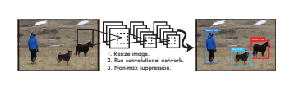
\includegraphics[width=0.47\textwidth]{D:/lecture/ITpaper/Access-Template/figure1.eps}
	\caption{\textbf{The YOLO Detection System.} Processing images with YOLO is simple and straightforward. Their system (1) resizes the input images to 448 x 448, (2) runs a single convolutional network on the image, and (3) thresholds the resulting detections by the model's confidence.}
	\label{fig:figure1}
\end{figure}

First, YOLO is extremely fast. The problem of obtaining the coordinates of the bounding box representing an object was to be optimized by combining the probability of the class with one. Even the Fast YOLO version achieved 150 fps in Titan X GPU environment. Even at this rate, they recorded twice as many precisions as the real-time object detection model at the time.
Second, YOLO model makes unseparated global inference. This way, they accelerated model speed at the implementation stage, using the C-language-based DarkNet framework that was created by the researchers themselves.
Third, YOLO learns generalizable representations of objects. When trained on natural images and tested on artwork, YOLO outperforms top detection methods like DPM and R-CNN by a wide margin. Since YOLO is highly generalizable it is less likely to break down when applied to new domains or unexpected outputs.


\subsection{Papers main idea or proposed idea}
They unify the separate components of object detection into a single neural network, end-to-end model. Their network uses features from the entire image to predict each bounding box and class probabilities. This means their network reasons globally about the full image and all the objects in the image.
Their system divides the input image into an S x S grid. They usually use 7 x 7 grid. If the center of an object falls into a grid cell, that grid cell is responsible for detecting that object. Each grid cell predicts B bounding boxes and confidence scores. They use intersection over union (IOU) to predict exact object. Formally, they define confidence as Pr(Object) * IOU. Each bounding box consists of 5 predictions: \textit{x, y, w, h}, and confidence. \eqref{eqaution1} shows this confidence.

\begin{equation}
	\label{equation1}
	\resizebox{.9\hsize}{!}{ \textit{Pr(Class_i}|Object) \ *\ Pr(Object)\ *\ IOU_{pred}^{truth} = Pr(Class_i)\ *\ IOU_{pred}^{truth}}
\end{equation}

Their network architecture i inspired by the GoogLeNet model for image classification. Their network has 24 convolutional layers followed by 2 fully connected layers. However, they simply use 1 x 1 reduction layers followed by 3 x 3 convolutional layers. The full network is shown in Figure \ref{fig:figure2}. Their final output is the 7 x 7 x 30 tensor of predictions.

\begin{figure*}
	\centering
		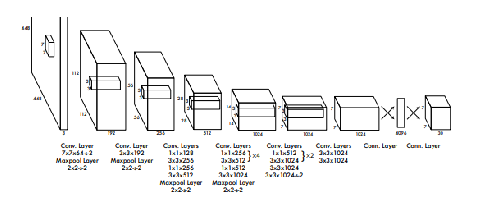
\includegraphics[width=1.00\textwidth]{D:/lecture/ITpaper/Access-Template/figure2.eps}
		\caption{\textbf{The Architecture.} Their detection network has 24 convolutional layers followed by 2 fully connected layers. Alternating 1 x 1 convolutional layers reduce the features space from preceding layers. They pretrain the convolutional layers on the ImageNet classification task at half the resolution (224 x 224 input image) and then double the resolution for detection.}
	\label{fig:figure2}
\end{figure*}

They pretrain their convolutional layers on the ImageNet 1000-class competition dataset. for pretraining they use the first 20 convolutional layers from Figure \ref{fig:figure2} followed by a average-pooling layer and a fully connectec layer. They then convert the model to perform detection. Detection often requires fine-grained visual information so they increase the input resolution of the network from 224 x 224 to 448 x 448.
Their final layer predicts both class probabilities and bounding box coordinates. They normalize the bounding box width and height by the image width and height so that they fall between 0 and 1. We parametrize the bounding box x and y coordinates to be offsets of a particular grid cell location so they are also bounded between 0 and 1. They use a linear activation function for the final layer and all other layers use the following leaky rectified linear activation:

\begin{equation}
	\label{equation2}
	 \phi(x) \ = \ \begin{cases} x, \ \ \ \ \ \ \ \  if \ x \ > \ 0 \\ 
	0.1x, \ \ \  otherwise
	\end{cases}
\end{equation}

They use sum-squared error because it is easy to optimize, however it does not perfectly align with our goal of
maximizing average precision. To remedy this, they increase the loss from bounding box coordinate predictions and decrease the loss from confidence predictions for boxes that don’t contain objects. They use two parameters, $\lambda_{coord}}$ and $\lambda_{noobj}$ to accomplish this. They set $\lambda_{coord} = 5$ and $\lambda_{noobj} = .5$. To partially address this they predict the square root of the bounding box width and height instead of the width and height directly.

\subsection{Results and discussions}
YOLO imposes strong spatial constraints on bounding box predictions since each grid cell only predicts two boxes and can only have one class. This spatial constraint limits the number of nearby objects that our model can predict. Our model struggles with small objects that appear in groups, such as flocks of birds. 
Since their model learns to predict bounding boxes from data, it struggles to generalize to objects in new or unusual aspect ratios or configurations. Their model also uses relatively coarse features for predicting bounding boxes since their architecture has multiple downsampling layers from the input image.
Finally, while they train on a loss function that approximates detection performance, our loss function treats errors the same in small bounding boxes versus large bounding boxes. A small error in a large box is generally benign but a small error in a small box has a much greater effect on IOU.

The recent Faster R-CNN replaces selective search with a neural network to propose bounding boxes, similar GoogLeNet. In their tests, their most accurate model achieves 7 fps while a smaller, less accurate one runs at 18 fps. The VGG-16 version of Faster R-CNN is 10 mAP higher but is also 6 times slower than YOLO. The ZFNet with Faster R-CNN is only 2.5 times slower than YOLO but is also less accurate.

\begin{table}[htb]
	\centering
	\renewcommand{\arraystretch}{1.2}
		\begin{tabular}{l r r r}
			 & mAP & Combined   & Gain\\
			\hline
			Fast R-CNN & 71.8 & - & - \\
			\hline
			Fast R-CNN (2007 data) & \textbf{66.9} & 72.4 & .6 \\
			Fast R-CNN (VGG-M) & 59.2 & 72.4 & .6 \\
			Fast R-CNN (CaffeNet) & 57.1 & 72.1 & .3 \\
			YOLO & 63.4 & \textbf{75.0} & \textbf{3.2} \\
		\end{tabular}
		\caption{\textbf{Model combination experiments on VOC 2007.} They examine the effect of combining various models with the best version of Fast R-CNN provide only a small benefit while YOLO provides a significant performance boost.}
	\label{Table_1}
\end{table}

The boost from YOLO is not simply a byproduct of model ensembling since there is little benefit from combining different versions of Fast R-CNN. Rather, it is precisely because YOLO makes different kinds of mistakes at test time that it is so effective at boosting Fast R-CNN’s performance.
Unfortunately, this combination doesn’t benefit from the speed of YOLO since we run each model seperately and then combine the results. However, since YOLO is so fast, it doesn’t add any significant computational time compared to Fast R-CNN.


\section{YOLO9000: Better, Faster, Stronger}
\subsection{Paper main Theme}
They introduce YOLO9000, a state-of-the-art, real-time object detection system that can detect over 9000 object categories. First we propose various improvements to the YOLO detection method, both novel and drawn from prior work. The improved model, YOLOv2, is state-of-the-art on standard detection tasks like PASCAL VOC and COCO. Using a novel, multi-scale training method the same YOLOv2 model can run at varying sizes, offering an easy tradeoff between speed and accuracy.
At 40 FPS, YOLOv2 gets 78.6 mAP, outperforming state-of-the-art methods like Faster RCNN with ResNet and SSD while still running significantly faster. They propose a method to jointly train on object detection and classification. Using this method they train YOLO9000 simultaneously on the COCO detection dataset and the ImageNet classification dataset. YOLO can detect more than just 200 classes; it predicts detections for more than 9000 different object categories. And it still runs in real-time.

They propose a new method to harness the large amount of classification data we already have and use it to expand the scope of current detection systems. Their method uses a hierarchical view of object classification that allows them to combine distinct datasets together.

They also propose a joint training algorithm that allows them to train object detectors on both detection and classification data. Their method leverages labeled detection images to learn to precisely localize objects while it uses classification images to increase its vocabulary and robustness.

YOLO suffers from a variety of shortcomings relative to state-of-the-art detection systems. Error analysis of YOLO compared to Fast R-CNN shows that YOLO makes a significant number of localization errors. Furthermore, YOLO has relatively low recall compared to region proposal-based methods. Thus they focus mainly on improving recall and localization while maintaining classification accuracy.

\subsection{Papers main idea or proposed idea}
Computer vision generally trends towards larger, deeper networks. Better performance often hinges on training larger networks or ensembling multiple models together. However, with YOLOv2 we want a more accurate detector that is still fast. Instead of scaling up their network, they simplify the network and then make the representation easier to learn. We pool a variety of ideas from past work with their own novel concepts to improve YOLO’s performance.

\textbf{Batch Normalization.} Batch normalization leads to significant improvements in convergence while eliminating the
need for other forms of regularization. By adding batch normalization on all of the convolutional layers in YOLO they get more than 2\% improvement in mAP.

\textbf{High Resolution Classifier.}  The original YOLO trains the classifier network at 224 × 224 and increases the resolution to 448 for detection. For YOLOv2 we first fine tune the classification network at the full 448 × 448 resolution for 10 epochs on ImageNet. This gives the network time to adjust its filters to work better on higher resolution input. They then fine tune the resulting network on detection. This high resolution classification network gives us an increase of almost 4\% mAP.

\textbf{Convolutional With Anchor Boxes.} YOLO predicts the coordinates of bounding boxes directly using fully connected layers on top of the convolutional feature extractor. Instead of predicting coordinates directly Faster R-CNN predicts bounding boxes using hand-picked priors. They remove the fully connected layers from YOLO and use anchor boxes to predict bounding boxes. When they move to anchor boxes they also decouple the class prediction mechanism from the spatial location and instead predict class and objectness for every anchor box.

Using anchor boxes they get a small decrease in accuracy. YOLO only predicts 98 boxes per image but with anchor boxes their model predicts more than a thousand. Without anchor boxes their intermediate model gets 69.5 mAP with a recall of 81\%. With anchor boxes our model gets 69.2 mAP with a recall of 88\%.

\textbf{Dimension Clusters.} They encounter two issues with anchor boxes when using them with YOLO. The first is that the box dimensions are hand picked. The network can learn to adjust the boxes appropriately but if they pick better priors for the network to start with we can make it easier for the network to learn to predict good detections.

Instead of choosing priors by hand, they run k-means clustering on the training set bounding boxes to automatically find good priors. Thus for their distance metric we use:

\begin{equation}
	\label{equation3}
	 d(box, centroid) \ = \ 1 - IOU(box, centroid) \\
\end{equation}

They run k-means for various values of k and plot the average IOU with closest centroid, see Figure \ref{fig:figure3}. They choose k = 5 as a good tradeoff between model complexity and high recall.

\begin{figure}
	\centering
		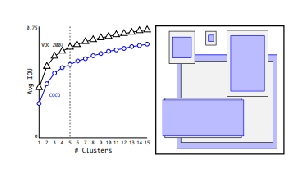
\includegraphics[width=0.47\textwidth]{D:/lecture/ITpaper/Access-Template/figure3.eps}
	\caption {\textbf{Clustering box dimensions on VOC and COCO.} They run k-means clustering on the dimensions of bounding boxes to get good priors for their model. The left image shows the average IOU they get with various choices for k. They find that k = 5 gives a good tradeoff for recall vs. complexity of the model. The right image shows the relative centroids for VOC and COCO. Both sets of priors favor thinner, taller boxes while COCO has greater variation in
size than VOC.}
	\label{fig:figure3}
\end{figure}

\textbf{Direct location prediction.} When using anchor boxes with YOLO we encounter a second issue: model instability, especially during early iterations. Most of the instability comes from predicting the (x, y) locations for the box.  In region proposal networks the network predicts values $t_x$ and $t_y$ and the $(x, y)$ center coordinates are calculated as:

\begin{equation}
	\label{equation4}
	\begin{split}
	 x \ & = \ (t_x \ * \ w_a) \ - \ x_a \\
	 y \ & = \ (t_y \ * \ h_a) \ - \ y_a
	\end{split}
\end{equation}

Since they constrain the location prediction the parametrization is easier to learn, making the network
more stable. Using dimension clusters along with directly predicting the bounding box center location improves YOLO by almost 5\% over the version with anchor boxes.

\textbf{Fine-Grained Features.} This modified YOLO predicts detections on a 13 × 13 feature map. Faster R-CNN and SSD both run their proposal networks at various feature maps in the network to get a range of resolutions. They take a different approach, simply adding a passthrough layer that brings features from an earlier layer at 26 × 26 resolution. The passthrough layer concatenates the higher resolution features with the low resolution features by stacking adjacent features into different channels instead of spatial locations, similar to the identity mappings in ResNet. 

\textbf{Multi-Scale Training.} since their model only uses convolutional and pooling layers it can be resized on the fly. We want YOLOv2 to be robust to running on images of different sizes so we train this into the model. They want YOLOv2 to be robust to running on images of different sizes so we train this into the model. Instead of fixing the input image size they change the network every few iterations. Every 10 batches their network randomly chooses a new image dimension size. they pull from the following multiples of 32.

\textbf{Darknet-19.} Most detection frameworks rely on VGG-16 as the base feature extractor. VGG-16 is a powerful, accurate classification network but it is needlessly complex. The convolutional layers of VGG-16 require 30.69 billion floating point operations for a single pass over a single image at 224 × 224 resolution. The YOLO framework uses a custom network based on the Googlenet architecture. This network is faster than VGG-16, only using 8.52 billion operations for a forward pass. However, it’s accuracy is slightly worse than VGG16. They propose a new classification model to be used as the base of YOLOv2. Their final model, called Darknet-19, has 19 convolutional layers and 5 maxpooling layers. For a full description see Table \ref{Table_2}.

\begin{table}[htb]
	\centering
	\scalebox{1}{%
		\begin{tabular}{c | c | c | c}
			Type & Filters & Size/Stride & Output\\
			\hline
			Convolutional & 32 & 3 x 3   & 224 x 224 \\
			Maxpool       &    & 2 x 2/2 & 112 x 112 \\
			Convolutional & 64 & 3 x 3   & 112 x 112 \\
			Maxpool       &    & 2 x 2/2 & 56 x 56 \\
			Convolutional & 128 & 3 x 3   & 56 x 56 \\			
			Convolutional & 64 & 1 x 1   & 56 x 56 \\
			Convolutional & 128 & 3 x 3   & 56 x 56 \\
			Maxpool       &    & 2 x 2/2 & 28 x 28 \\			
			Convolutional & 256 & 3 x 3   & 28 x 28 \\			
			Convolutional & 128 & 1 x 1   & 28 x 28 \\
			Convolutional & 256 & 3 x 3   & 28 x 28 \\
			Maxpool       &    & 2 x 2/2 & 14 x 14 \\	
			Convolutional & 512 & 3 x 3   & 14 x 14 \\
			Convolutional & 256 & 1 x 1   & 14 x 14 \\	
			Convolutional & 512 & 3 x 3   & 14 x 14 \\	
			Convolutional & 256 & 1 x 1   & 14 x 14 \\
			Convolutional & 512 & 3 x 3   & 14 x 14 \\
			Maxpool       &    & 2 x 2/2 & 7 x 7 \\
			Convolutional & 1024 & 3 x 3   & 7 x 7 \\
			Convolutional & 512 & 1 x 1   & 7 x 7 \\
			Convolutional & 1024 & 3 x 3   & 7 x 7 \\
			Convolutional & 512 & 1 x 1   & 7 x 7 \\
			Convolutional & 1024 & 3 x 3   & 7 x 7 \\
			\hline
			\hline
			Convolutional & 1000 & 1 x 1   & 7 x 7 \\
			Avgpool &  & Global & 1000 \\
			softmax & & & \\
		\end{tabular}}
		\caption{\textbf{Darknet-19.}}
	\label{Table_2}
\end{table}

\textbf{Joint classification and detection.} Now that they can combine datasets using WordTree they can train our joint model on classification and detection. We want to train an extremely large scale detector so they create our combined dataset using the COCO detection dataset and the top 9000 classes from the full ImageNet release. The corresponding WordTree for this dataset has 9418 classes.

When it sees a classification image they only backpropagate classification loss. To do this they simply find the bounding box that predicts the highest probability for that class and they compute the loss on just its predicted tree.

\begin{figure}
	\centering
		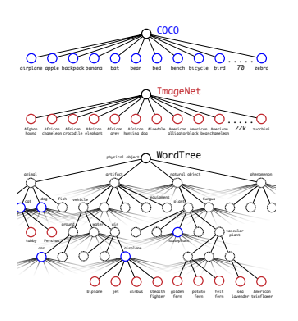
\includegraphics[width=0.47\textwidth]{D:/lecture/ITpaper/Access-Template/figure4.eps}
	\caption {\textbf{Combining datasets using WordTree hierarchy.} Using the WordNet concept graph we build a hierarchical tree of visual concepts. Then they can merge datasets together by mapping the classes in the dataset to synsets in the tree. This is a simplified view of WordTree for illustration purposes.}
	\label{fig:figure4}
\end{figure}

\subsection{Results and discussions}
YOLO9000 is a real-time framework for detection more than 9000 object categories by jointly optimizing detection and classification. We use WordTree to combine data from various sources and our joint optimization technique to train simultaneously on ImageNet and COCO. Many of their techniques generalize outside of object detection. Their WordTree representation of ImageNet offers a richer, more detailed output space for image classification.

\section{YOLOv3: An Incremental Improvement}
\subsection{Paper main Theme}
They present some updates to YOLO! They made a bunch of little design changes to make it better. They also trained this new network that’s pretty swell. It’s a little bigger than last time, YOLOv2, but more accurate. It achieves 57.9 AP50 in 51 ms on a Titan X, compared to 57.5 AP50 in 198 ms by RetinaNet, simila performance but 3.8× faster.

Following YOLO9000 their system predicts bounding boxes using dimension clusters as anchor boxes [15]. The network predicts 4 coordinates for each bounding box, $t_x$, $t_y$, $t_w$, $t_h$. If the cell is offset from the top left corner of the image by $(c_x, c_y)$ and the bounding box prior has width and height $p_w$, $p_h$, then the predictions correspond to:

\begin{equation}
	\label{equation5}
	\begin{split}
	 b_x \ & = \ \sigma(t_x) \ + \ c_x \\
	 b_y \ & = \ \sigma(t_y) \ + \ c_y \\
	b_w \ & = \ p_w e^{t_w} \\
	b_h \ & = \ p_h e^{t_h} \\
	\end{split}
\end{equation}

During training they use sum of squared error loss. If the ground truth for some coordinate prediction is $tˆ*$ their gradient is the ground truth value (computed from the ground truth box) minus their prediction: $tˆ* − t*$. This ground truth value can be easily computed by inverting the equations above. YOLOv3 predicts an objectness score for each bounding box using logistic regression. This should be 1 if the bounding box prior overlaps a ground truth object by more than any other bounding box prior.

\begin{figure}
	\centering
		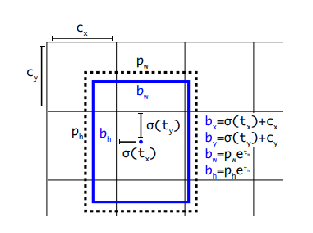
\includegraphics[width=0.47\textwidth]{D:/lecture/ITpaper/Access-Template/figure5.eps}
	\caption {\textbf{Bounding boxes with dimension priors and location prediction.} They predict the width and height of the box as offsets from cluster centroids. We predict the center coordinates of the box relative to the location of filter application using a sigmoid function. This figure blatantly self-plagiarized from.}
	\label{fig:figure5}
\end{figure}

\subsection{Papers main idea or proposed idea}
Each box predicts the classes the bounding box may contain using multilabel classification. They do not use a softmax as they have found it is unnecessary for good performance, instead they simply use independent logistic classifiers. During training they use binary cross-entropy loss for the class predictions. This formulation helps when they move to more complex domains like the Open Images Dataset.

YOLOv3 predicts boxes at 3 different scales. Their system extracts features from those scales using a similar concept to feature pyramid networks. From their base feature extractor they add several convolutional layers. The last of these predicts a 3-d tensor encoding bounding box, objectness, and class predictions. they predict 3 boxes at each scale so the tensor is $N$ x $N$ x $3 \ * \ (4 \ + \ 1 \ + \ 80)$ for the 4 bounding box offsets, 1 objectness prediction, and 80 class predictions.

They also take a feature map from earlier in the network and merge it with their upsampled features using concatenation. This method allows us to get more meaningful semantic information from the upsampled features and finer-grained information from the earlier feature map. They then add a few more convolutional layers to process this combined feature map, and eventually predict a similar tensor, although now twice the size.

They still use k-means clustering to determine their bounding box priors. They just sort of chose 9 clusters and 3 scales arbitrarily and then divide up the clusters evenly across scales.

They use a new network for performing feature extraction. Their new network is a hybrid approach between the network used in YOLOv2, Darknet-19, and that newfangled residual network stuff. Their network uses successive 3 × 3 and 1 × 1 convolutional layers but now has some shortcut connections as well and is significantly larger. It has 53 convolutional layers so call it Darknet-53.

This new network is much more powerful than Darknet19 but still more efficient than ResNet-101 or ResNet-152. Here are some ImageNet results:

\begin{table}[htb]
	\centering
	\renewcommand{\arraystretch}{1.2}
	\scalebox{1}{%
		\begin{tabular}{l r r r r r}
			Backbone & Top-1 & Top-5 & Bn Ops & BFLOP/s & FPS \\
			\hline
			Darknet-19 & 74.1 & 91.8 & 7.29 & 1246 & \textbf{171} \\
			ResNet-101 & 77.1 & 93.7 & 19.7 & 1039 & 53 \\
			ResNet-152 & \textbf{77.6} & \textbf{93.8} & 29.4 & 1090 & 37 \\
			ResNet-101 & 77.2 & \textbf{93.8} & 18.7 & \textbf{1457} & 78 \\
		\end{tabular}}
		\caption{\textbf{Comparison of backbones.} Accuracy, billions of operations, billion floating point operations per second, and FPS for various networks.}
	\label{Table_3}
\end{table}

In terms of COCOs weird average mean AP metric it is on par with the SSD variants but is 3× faster. However, when they look at the “old” detection metric of
mAP at IOU $= \ .5$ (or $AP_50$ in the chart) YOLOv3 is very strong. It is almost on par with RetinaNet and far above the SSD variants. This indicates that YOLOv3 is a very strong detector that excels at producing decent boxes for objects. However, performance drops significantly as the IOU threshold increases indicating YOLOv3 struggles to get the boxes perfectly aligned with the object.

In the past YOLO struggled with small objects. However, now they see a reversal in that trend. With the new multi-scale predictions we see YOLOv3 has relatively high
APS performance.

They tried lots of stuff while they were working on YOLOv3. A lot of it didn’t work. Here’s the stuff they can remember.

\textbf{Anchor box x, y offset predictions.} They tried using the normal anchor box prediction mechanism where you predict the x, y offset as a multiple of the box width or height using a linear activation. They found this formulation decreased model stability and didn’t work very well. Linear x, y predictions instead of logistic. They tried using a linear activation to directly predict the x, y offset instead of the logistic activation. This led to a couple point drop in mAP. 

\textbf{Focal loss.} They tried using focal loss. It dropped their mAP about 2 points. YOLOv3 may already be robust to the problem focal loss is trying to solve because it has separate objectness predictions and conditional class predictions. Thus for most examples there is no loss from the class predictions? Or something? They aren’t totally sure.

\textbf{Dual IOU thresholds and truth assignment.} Faster RCNN uses two IOU thresholds during training. If a prediction overlaps the ground truth by .7 it is as a positive example, by [.3−.7] it is ignored, less than $.3$ for all ground truth objects it is a negative example. We tried a similar strategy but couldn’t get good results. They quite like our current formulation, it seems to be at a local optima at least. It is possible that some of these techniques could eventually produce good results, perhaps they just need some tuning to stabilize the training.

\begin{figure*}
	\centering
		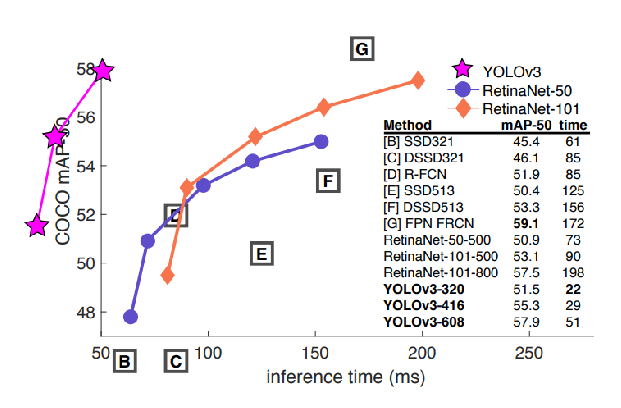
\includegraphics[width=0.98\textwidth]{D:/lecture/ITpaper/Access-Template/figure6.eps}
	\caption {Again adapted from the, this time displaying speed/accuracy tradeoff on the mAP at $.5$ IOU metric. You can tell YOLOv3 is good because it’s very high and far to the left. They also fix a data loading bug in YOLOv2, that helped by like 2 mAP.}
	\label{fig:figure6}
\end{figure*}

\subsection{Results and discussions}
YOLOv3 is a good detector. It’s fast, it’s accurate. It’s not as great on the COCO average AP between $.5$ and $.95$ IOU metric. But it’s very good on the old detection metric of $.5$ IOU. As Figure \ref{fig:figure6}, YOLOv3 has good performance compared to SSD, RetinaNet.


\section{SSD: Single Shot MultiBox Detector}
\subsection{Paper main Theme}
They present a method for detecting objects in images using a single deep neural network. Their approach, named SSD, discretizes the output space of
bounding boxes into a set of default boxes over different aspect ratios and scales per feature map location. At prediction time, the network generates scores for the
presence of each object category in each default box and produces adjustments to the box to better match the object shape. Additionally, the network combines predictions from multiple feature maps with different resolutions to naturally handle objects of various sizes. SSD is simple relative to methods that require object
proposals because it completely eliminates proposal generation and subsequent pixel or feature resampling stages and encapsulates all computation in a single network.

While Faster R-CNN is accurate, albeit with deeper features, this approach had been too computationally intensive for embedded systems and, even with high-end hardware, too slow for real-time applications, operatiing at only 7 frames per second (FPS).

This paper presents the first deep network based object detector that does not resample pixels or features for bounding box hypotheses and and is as accurate as approaches that do. This results in a significant improvement in speed for high-accuracy detection (59 FPS with mAP 74.3\% on VOC2007 test, vs. Faster R-CNN 7 FPS with mAP 73.2\% or YOLO 45 FPS with mAP 63.4\%). The fundamental improvement in speed comes from eliminating bounding box proposals and the subsequent pixel or feature resampling stage.

They are not the first to do this such as YOLO, but by adding a series of improvements, they manage to increase the accuracy significantly over previous attempts. Their improvements include using a small convolutional filter to predict object categories and offsets in bounding box locations, using separate predictors (filters) for different aspect ratio detections, and applying these filters to multiple feature maps from the later stages of a network in order to perform detection at multiple scales.

– They introduce SSD, a single-shot detector for multiple categories that is faster than the previous model for single shot detectors (YOLO), and significantly
more accurate, in fact as accurate as slower techniques that perform explicit region proposals and pooling (including Faster R-CNN).

– The core of SSD is predicting category scores and box offsets for a fixed set of default bounding boxes using small convolutional filters applied to feature maps.

– To achieve high detection accuracy we produce predictions of different scales from feature maps of different scales, and explicitly separate predictions by aspect ratio.

– These design features lead to simple end-to-end training and high accuracy, even on low resolution input images, further improving the speed vs accuracy trade-off.

– Experiments include timing and accuracy analysis on models with varying input size evaluated on PASCAL VOC, COCO, and ILSVRC and are compared to a range of recent state-of-the-art approaches.

\begin{figure}
	\centering
		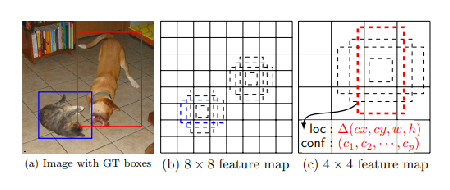
\includegraphics[width=0.47\textwidth]{D:/lecture/ITpaper/Access-Template/figure7.eps}
	\caption {\textbf{SSD framework.} (a) SSD only needs an input image and ground truth boxes for each object during training. In a convolutional fashion, they evaluate a small set of default boxes of different aspect ratios at each location in several feature maps with different scales (e.g. 8 × 8 and 4 × 4 in (b) and (c)). For each default box, they predict both the shape offsets and the confidences for all object categories (($c_1$, $c_2$, · · · , $c_p$)). At training time, they first match these default boxes to the ground truth boxes. For example, they have matched two default boxes with the cat and one with the dog, which are treated as positives and the rest as negatives. The model loss is a weighted sum between localization loss (e.g. Smooth L1) and confidence loss (e.g. Softmax).}
	\label{fig:figure7}
\end{figure}

\subsection{Papers main idea or proposed idea}

\begin{figure*}
	\centering
		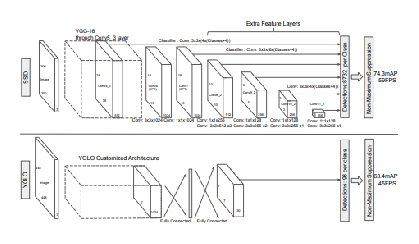
\includegraphics[width=0.90\textwidth]{D:/lecture/ITpaper/Access-Template/figure8.eps}
	\caption {A comparison between two single shot detection models: SSD and YOLO. Their SSD model adds several feature layers to the end of a base network, which predict the offsets to default boxes of different scales and aspect ratios and their associated confidences. SSD with a 300 × 300 input size significantly outperforms its 448 × 448 YOLO counterpart in accuracy on VOC2007 test while also improving the speed.}
	\label{fig:figure8}
\end{figure*}

The SSD approach is based on a feed-forward convolutional network that produces a fixed-size collection of bounding boxes and scores for the presence of object class
instances in those boxes, followed by a non-maximum suppression step to produce the final detections. They use the VGG-16 network as a base, but other networks should also produce good results. They then add auxiliary structure to the network to produce detections with the following key features:

\textbf{Multi-scale feature maps for detection.} They add convolutional feature layers to the end of the truncated base network. These layers decrease in size progressively and allow predictions of detections at multiple scales.

\textbf{Convolutional predictors for detection.} Each added feature layer (or optionally an existing feature layer from the base network) can produce a fixed set of detection predictions using a set of convolutional filters. These are indicated on top of the SSD network architecture in Figure \ref{fig:figure8}. The bounding box offset output values are measured relative to a default box position relative to each feature map location.

\textbf{Default boxes and aspect ratios.} They associate a set of default bounding boxes with each feature map cell, for multiple feature maps at the top of the network. The default boxes tile the feature map in a convolutional manner, so that the position of each box relative to its corresponding cell is fixed. At each feature map cell, they predict the offsets relative to the default box shapes in the cell, as well as the per-class scores that indicate the presence of a class instance in each of those boxes. They compute $c$ class scores and the 4 offsets relative to the original default box shape. This results in a total of $(c + 4)^k$ filters that are applied around each location in the feature map, yielding $(c + 4)^{kmn}$ outputs for a m × n feature map.

The SSD training objective is derived from the MultiBox objective [7,8] but is extended to handle multiple object categories. Let $x^{p}_{ij} / = / ${1, 0} be an indicator for matching the $i$-th default box to the $j$-th ground truth box of category $p$. In the matching strategy above, we can have $\sum P_i x^{p}_{ij} \ \geq \ 1$. The overall objective loss function is a weighted sum of the localization loss (loc) and the confidence loss (conf):

\begin{equation}
	\label{equation6}
	 L(x, \ c, \ l, \ g) \ = \ \frac{1}{N} (L_{conf}(x, c) \ + \ \alpha L_{loc}(x,l,g))
\end{equation}

Their experiments are all based on VGG16, which is pre-trained on the ILSVRC CLS-LOC dataset. Similar to DeepLab-LargeFOV, they convert
fc6 and fc7 to convolutional layers, subsample parameters from fc6 and fc7, change pool5 from 2 × 2 $− s2$ to 3 × 3 $− s1$, and use the $\acute{a} trous$ algorithm  to fill the ”holes”. They remove all the dropout layers and the fc8 layer. They fine-tune the resulting model using SGD with initial learning rate $10^{-3}$, 0.9 momentum, 0.0005 weight decay, and batch size 32.

\subsection{Results and discussions}

To understand SSD better, they carried out controlled experiments to examine how each component affects performance.

\textbf{Data augmentation is crucial.} Fast and Faster R-CNN use the original image and the horizontal flip to train. They use a more extensive sampling strategy, similar to YOLO. They can improve 8.8\% mAP with this sampling strategy.

\textbf{More default box shapes is better.} By default they use 6 default boxes per location. If we remove the boxes with $\prac{1}{3}$ and 3 aspect ratios, the
performance drops by 0.6\%.

\textbf{Atrous is faster.} They used the atrous version of a subsampled VGG16, following DeepLab-LargeFOV. The result is about the same while the speed is about 20\% slower.

\textbf{Multiple output layers at different resolutions is better.} A major contribution of SSD is using default boxes of different scales on different output layers. To measure the advantage gained, we progressively remove layers and compare results. The SSD architecture combines predictions from feature maps of various resolutions to achieve comparable accuracy to Faster R-CNN, while using lower resolution input images.

Considering the large number of boxes generated from our method, it is essential to perform non-maximum suppression (nms) efficiently during inference. By using a confidence threshold of 0.01, they can filter out most boxes.

\begin{table}[htb]
	\centering
	\renewcommand{\arraystretch}{1.2}
	\scalebox{0.8}{%
		\begin{tabular}{l | c | c | c | c | c}
			Mehtod & mAP & FPS & batch size & # Boxes & Input resolution \\
			\hline
			Faster R-CNN (VGG16) & 73.2 & 7 & 1 & $\sim$ 6000 & $\sim$ 1000 x 600 \\
			\hline
			Fast YOLO & 52.7 & 155 & 1 & 98 & 448 x 448 \\
			YOLO (VGG16) & 66.4 & 21 & 1 & 98 & 448 x 448 \\
			\hline
			SSD300 & 74.3 & 46 & 1 & 8732 & 300 x 300 \\
			SSD512 & 76.8 & 19 & 1 & 24564 & 512 x 512 \\
			SSD300 & 74.3 & 59 & 1 & 8732 & 300 x 300 \\
			SSD512 & 76.8 & 22 & 1 & 24564 & 512 x 512 \\
		\end{tabular}}
		\caption{\textbf{Results on Pascal VOC2007 test.} SSD300 is the only real-time detection method that can achieve above 70\% mAP. By using a larger input image, SSD512 outperforms all methods on accuracy while maintaining a close to real-time speed.}
	\label{Table_4}
\end{table}

This paper introduces SSD, a fast single-shot object detector for multiple categories. A key feature of our model is the use of multi-scale convolutional bounding box outputs attached to multiple feature maps at the top of the network. This representation allows them to efficiently model the space of possible box shapes. They demonstrate that given the same VGG-16 base architecture, SSD compares favorably to its state-of-the-art object detector counterparts in terms of both accuracy and speed.

\section{MobileNets: Efficient Convolutional Neural Networks for Mobile Vision Applications}
\subsection{Paper main Theme}
They present a class of efficient models called MobileNets for mobile and embedded vision applications. MobileNets are based on a streamlined architecture that uses depthwise separable convolutions to build light weight deep neural networks. They introduce two simple global hyperparameters that efficiently trade off between latency and accuracy. These hyper-parameters allow the model builder to choose the right sized model for their application based on the constraints of the problem.

This paper describes an efficient network architecture and a set of two hyper-parameters in order to build very small, low latency models that can be easily matched to the design requirements for mobile and embedded vision applications. MobileNet architecture and two hyper-parameters width multiplier and resolution multiplier.  to define smaller and more efficient MobileNets. 

This paper proposes a class of network architectures that allows a model developer to specifically choose a small network that matches the resource restrictions (latency, size) for their application. MobileNets primarily focus on optimizing for latency but also yield small networks. Many papers on small networks focus only on size but do not consider speed.

MobileNets are built primarily from depthwise separable convolutions initially introduced in Xception and subsequently used in Inception models to reduce the computation in the first few layers. Factorized Networks introduces a similar factorized convolution as well as the use of topological connections. Subsequently, the Xception network demonstrated how to scale up depthwise separable filters to out perform Inception V3 networks.

A different approach for obtaining small networks is shrinking, factorizing or compressing pretrained networks. Compression based on product quantization, hashing, and pruning, vector quantization and Huffman coding have been proposed in the literature. It is complementary to their approach and is covered in some of their use cases.

\subsection{Papers main idea or proposed idea}
The MobileNet model is based on depthwise separableb convolutions which is a form of factorized convolutions which factorize a standard convolution into a depthwise convolution and a 1×1 convolution called a pointwise convolution. For MobileNets the depthwise convolution applies a single filter to each input channel. The pointwise convolution then applies a 1×1 convolution to combine the outputs the depthwise convolution. The depthwise separable convolution splits this into two layers, a separate layer for filtering and a separate layer for combining. This factorization has the effect of drastically reducing computation and model size.  Figure \ref{fig:figure9} shows how a standard convolution 2$(a)$ is factorized into a depthwise convolution 2$(b)$ and a 1 × 1 pointwise convolution 2$(c)$.

\begin{figure}
	\centering
		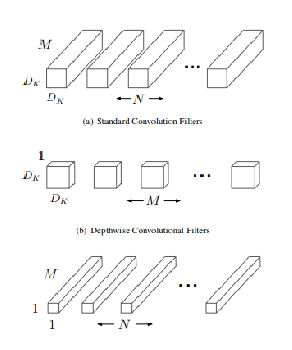
\includegraphics[width=0.47\textwidth]{D:/lecture/ITpaper/Access-Template/figure9.eps}
	\caption {The standard convolutional filters in $(a)$ are replaced by two layers: depthwise convolution in $(b)$ and pointwise convolution in $(c)$ to build a depthwise separable filter.}
	\label{fig:figure9}
\end{figure}

Depthwise separable convolution are made up of two layers: depthwise convolutions and pointwise convolutions. They use depthwise convolutions to apply a single filter per each input channel (input depth). Pointwise convolution, a simple 1×1 convolution, is then used to create a linear combination of the output of the depthwise layer. MobileNets use both batchnorm and ReLU nonlinearities for both layers. Depthwise separable convolutions cost:

\begin{equation}
	\label{equation7}
	 D_K \cdot D_K \cdot M \cdot D_F \cdot D_F \ + \ M \cdot N \cdot D_F \cdot D_F 
\end{equation}

MobileNet uses 3 × 3 depthwise separable convolutions which uses between 8 to 9 times less computation than standard convolutions at only a small reduction in accuracy.

The MobileNet structure is built on depthwise separable convolutions as mentioned in the previous section except for the first layer which is a full convolution.  All layers are followed by a batchnorm and ReLU nonlinearity with the exception of the final fully connected layer which has no nonlinearity and feeds into a softmax layer for classification. Counting depthwise and pointwise convolutions as separate layers, MobileNet has 28 layers.

MobileNet models were trained in TensorFlow using RMSprop with asynchronous gradient descent similar to Inception V3. However, contrary to training large models we use less regularization and data augmentation techniques because small models have less trouble with overfitting.

\begin{table}[htb]
	\centering
	\renewcommand{\arraystretch}{1.1}
	\caption{MobileNet Body Architecture}
	\scalebox{1}{%
		\begin{tabular}{l | l | l}
			\hline
			\hline
			Type / Stride & Filter Shape & Input Size \\
			\hline
			Conv / s2 &  3 x 3 x 3 x 32 & 224 x 224 x 3 \\
			\hline
			Conv dw / s1 &  3 x 3 x 32 dw & 112 x 112 x 32 \\
			\hline
			Conv / s2 &  1 x 1 x 32 x 64 & 112 x 112 x 32 \\
			\hline
			Conv dw / s2 &  3 x 3 x 64 dw & 112 x 112 x 64 \\
			\hline
			Conv / s1 &  1 x 1 x 64 x 128 & 56 x 56 x 64 \\
			\hline
			Conv dw / s1 &  3 x 3 x 128 dw & 56 x 56 x 128 \\
			\hline
			Conv / s1 &  1 x 1 x 128 x 128 & 56 x 56 x 128 \\
			\hline
			Conv dw / s2 &  3 x 3 x 128 dw & 56 x 56 x 128 \\
			\hline
			Conv / s1 &  1 x 1 x 256 x 256 & 28 x 28 x 128 \\
			\hline
			Conv dw / s1 &  3 x 3 x 256 dw & 28 x 28 x 256 \\
			\hline
			Conv / s1 &  1 x 1 x 256 x 256 & 28 x 28 x 256 \\
			\hline
			Conv dw / s2 &  3 x 3 x 256 dw & 28 x 28 x 256 \\
			\hline
			Conv / s1 &  1 x 1 x 256 x 512 & 14 x 14 x 256 \\
			\hline
			\multirow{2}{*}{5x}
				Conv dw / s1 & 3 x 3 x 512 dw & 14 x 14 x 512 \\
			\ \	\ \ \ Conv / s1	 & 1 x 1 x 512 x 512 & 14 x 14 x 512 \\
			\hline
			Conv dw / s2 &  3 x 3 x 512 dw & 14 x 14 x 512 \\
			\hline
			Conv / s1 &  1 x 1 x 512 x 1024 & 7 x 7 x 512 \\
			\hline
			Conv dw / s2 &  3 x 3 x 1024 dw & 7 x 7 x 1024 \\
			\hline
			Conv / s1 &  1 x 1 x 1024 x 1024 & 7 x 7 x 1024 \\
			\hline
			Avg Pool / s1 & Pool 7 x 7 & 7 x 7 x 1024 \\
			\hline
			FC / s1 &  1024 x 1000 & 1 x 1 x 1024 \\
			\hline
			softmax / s1 &  Classifier & 1 x 1 x 1000 \\
			\hline
		\end{tabular}}
		
	\label{Table_5}
\end{table}

\subsection{Results and discussions}

MobileNet can also be deployed as an effective base network in modern object detection systems. They report results for MobileNet trained for object detection on COCO data based on the recent work that won the 2016 COCO challenge.  MobileNet is compared to VGG and Inception V2 under both Faster-RCNN and SSD framework. In their experiments, SSD is evaluated with 300 input resolution (SSD 300) and Faster-RCNN is compared with both 300 and 600 input resolution (FasterRCNN 300, Faster-RCNN 600). The Faster-RCNN model evaluates 300 RPN proposal boxes per image. The models are trained on COCO train+val excluding 8k minival images and evaluated on minival. For both frameworks, MobileNet achieves comparable results to other networks with only a fraction of computational complexity and model size.

\begin{figure}
	\centering
		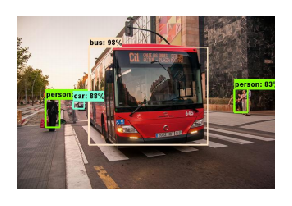
\includegraphics[width=0.47\textwidth]{D:/lecture/ITpaper/Access-Template/figure10.eps}
	\caption { Example objection detection results using MobileNet SSD.}
	\label{fig:figure10}
\end{figure}

They proposed a new model architecture called MobileNets based on depthwise separable convolutions. They investigated some of the important design decisions leading
to an efficient model. We then demonstrated how to build smaller and faster MobileNets using width multiplier and resolution multiplier by trading off a reasonable amount of accuracy to reduce size and latency.


\section{Conclusion}

In this paper, we summarized and compared the most popular real-time object detection CNN model, YOLO and SSD. The two models came out at the same time, 2016 and were both real-time and accurate in their own way. Both models commonly wanted to reduce region proposal cost, of the existing Fast-RCN, Faster-RCN. Nevertheless, the end-to-end model of train and test was maintained.

Both models, although similar for common purposes, looked different in detail. YOLO uses DarkNet to perform Feature Detection and then create a Conv Layer. However, the Multi-scale feature map is not used to detect it independently. Instead, it is partially flattened and connected to other low resolution maps. For example, YOLO reshape 28x28x512 Layer to 14x14x2048. It is then connected to the 14x14x1024 Feature map. YOLO then makes predictions by applying the Conv filter to the new 14x14x3072 layer. YOLov2 improved implementation of mAP from 63.4 to 78.6 for the first release. YOLO9000 can detect 9,000 different categories of objects.

YOLOv3 is changed to a more complex backbone for Feature extraction. Darknet-53 consists mainly of 3x3 and 1x1 filters that use skipped connections, such as ResNet's remaining network. Darknet-53 has less BFLOP (Billion Floating Point OPERATION) than ResNet-152 but has the same classification accuracy at twice the speed. YOLOv3 added Feature Pyramid to better detect small subjects. There is a tradeoff between accuracy and speed for different detectors.

SSD is a single-shot detector that uses the VGG19 network as a Feature Extractor (same as CNN on Master R-CNN) and predicts object classes later with a custom Conv Layer and using Conv filter. (However, Conv Layer reduces spatial dimensions and resolution.) Therefore, the above model can only detect large objects. To solve this problem, they detect an independent object in the Multiple Feature map. SSD uses existing layers in the Conv network to detect objects. It should be noted that redrawing the diagram close to scale has greatly reduced spatial resolution, and is missing the opportunity to find small objects that are too difficult to detect at low resolution. If you have this problem, you should increase the resolution of the input image.

In terms of user use, both models have advantages and disadvantages. First of all, YOLO has its own framework, C language-based Darknet, which has significant advantages in computational cost. However, it is difficult to apply frameworks to Python language, the most common language in deep learning.

In contrast, SSD offer API in Google's development framework, Tensorflow, which makes it quite easy to run in a Python environment. This can be easily implemented in Windows environment. Also, the model's architecture has the advantage of being easy to put on another CNN model. More recently, Google has developed MobileNet v2, which offers significant advantages in terms of speed and memory. Another strength is that Google continues to make innovative research into CNN.

Of course, YOLO has made a lot of progress from v1 to v3 so far, YOLO's popularity has been higher than SSD. From a user perspective, the best model would be to pinpoint the problem that needs to be solved with deep learning, calculate the cost to solve the problem, and select the best model in the limited resources. So far, the speed is YOLO, the accuracy is the stronger side of SSD, but this is also different from dataset, so the most important thing is to choose the best model in your own world.

\begin{thebibliography}{00}

\bibitem{b1} J. Redmon, S. Divvala, R. Girshick, A. Farhadi, ``You only look once: Unified, real-time object detection,'' in \emph{CVPR}, 2016.

\bibitem{b2} J. Redmon and A. Farhadi, ``Yolo9000: Better, faster, stronger,'' in \emph{n Computer Vision and Pattern Recognition (CVPR)},  2017 IEEE Conference on,, pp. 6517–6525, IEEE, 2017.

\bibitem{b3} J. Redmon and A. Farhadi, ``Yolov3: An incremental improvement,'' \emph{arXiv}, 2018.

\bibitem{b4} W. Liu, D. Anguelov, D. Erhan, C. Szegedy, S. Reed, C.Y. Fu, and A. C. Berg, ``SSD: Single shot multibox detector,'' in \emph{European conference on computer vision}, pp. 21-37. Springer, 2016.

\bibitem{b5} A. G. Howard, M. Zhu, B. Chen, D. Kalenichenko, W. Wang, T. Weyand, M. Andreetto, and H. Adam, ``Mobilenets: Efficient convolutional neural networks for mobile vision applications.,'' \emph{CoRR}., abs/1704.04861, 2017.

\end{thebibliography}

\begin{IEEEbiography}[{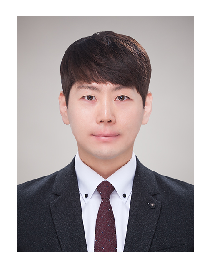
\includegraphics[width=1in, height=1.25in,clip,keepaspectratio]{JHS2.eps}}]{Hyeon Seong Jeon}
was born in Seoul, Korea in 1990. He received the B.E. degree in mass communication and journalism from Sungkyunkwan University (SKKU) Seoul, in 2017. In 2019, he joined the Department of Artificial Intelligence from Sunkyunkwan University, Suwon. His current research interests include A.I. and self-driving car using Deep learning.
\end{IEEEbiography}



\EOD

\end{document}
